\documentclass[twoside]{book}

% Packages required by doxygen
\usepackage{fixltx2e}
\usepackage{calc}
\usepackage{doxygen}
\usepackage[export]{adjustbox} % also loads graphicx
\usepackage{graphicx}
\usepackage[utf8]{inputenc}
\usepackage{makeidx}
\usepackage{multicol}
\usepackage{multirow}
\PassOptionsToPackage{warn}{textcomp}
\usepackage{textcomp}
\usepackage[nointegrals]{wasysym}
\usepackage[table]{xcolor}

% Font selection
\usepackage[T1]{fontenc}
\usepackage[scaled=.90]{helvet}
\usepackage{courier}
\usepackage{amssymb}
\usepackage{sectsty}
\renewcommand{\familydefault}{\sfdefault}
\allsectionsfont{%
  \fontseries{bc}\selectfont%
  \color{darkgray}%
}
\renewcommand{\DoxyLabelFont}{%
  \fontseries{bc}\selectfont%
  \color{darkgray}%
}
\newcommand{\+}{\discretionary{\mbox{\scriptsize$\hookleftarrow$}}{}{}}

% Page & text layout
\usepackage{geometry}
\geometry{%
  a4paper,%
  top=2.5cm,%
  bottom=2.5cm,%
  left=2.5cm,%
  right=2.5cm%
}
\tolerance=750
\hfuzz=15pt
\hbadness=750
\setlength{\emergencystretch}{15pt}
\setlength{\parindent}{0cm}
\setlength{\parskip}{3ex plus 2ex minus 2ex}
\makeatletter
\renewcommand{\paragraph}{%
  \@startsection{paragraph}{4}{0ex}{-1.0ex}{1.0ex}{%
    \normalfont\normalsize\bfseries\SS@parafont%
  }%
}
\renewcommand{\subparagraph}{%
  \@startsection{subparagraph}{5}{0ex}{-1.0ex}{1.0ex}{%
    \normalfont\normalsize\bfseries\SS@subparafont%
  }%
}
\makeatother

% Headers & footers
\usepackage{fancyhdr}
\pagestyle{fancyplain}
\fancyhead[LE]{\fancyplain{}{\bfseries\thepage}}
\fancyhead[CE]{\fancyplain{}{}}
\fancyhead[RE]{\fancyplain{}{\bfseries\leftmark}}
\fancyhead[LO]{\fancyplain{}{\bfseries\rightmark}}
\fancyhead[CO]{\fancyplain{}{}}
\fancyhead[RO]{\fancyplain{}{\bfseries\thepage}}
\fancyfoot[LE]{\fancyplain{}{}}
\fancyfoot[CE]{\fancyplain{}{}}
\fancyfoot[RE]{\fancyplain{}{\bfseries\scriptsize Generated by Doxygen }}
\fancyfoot[LO]{\fancyplain{}{\bfseries\scriptsize Generated by Doxygen }}
\fancyfoot[CO]{\fancyplain{}{}}
\fancyfoot[RO]{\fancyplain{}{}}
\renewcommand{\footrulewidth}{0.4pt}
\renewcommand{\chaptermark}[1]{%
  \markboth{#1}{}%
}
\renewcommand{\sectionmark}[1]{%
  \markright{\thesection\ #1}%
}

% Indices & bibliography
\usepackage{natbib}
\usepackage[titles]{tocloft}
\setcounter{tocdepth}{3}
\setcounter{secnumdepth}{5}
\makeindex

% Hyperlinks (required, but should be loaded last)
\usepackage{ifpdf}
\ifpdf
  \usepackage[pdftex,pagebackref=true]{hyperref}
\else
  \usepackage[ps2pdf,pagebackref=true]{hyperref}
\fi
\hypersetup{%
  colorlinks=true,%
  linkcolor=blue,%
  citecolor=blue,%
  unicode%
}

% Custom commands
\newcommand{\clearemptydoublepage}{%
  \newpage{\pagestyle{empty}\cleardoublepage}%
}

\usepackage{caption}
\captionsetup{labelsep=space,justification=centering,font={bf},singlelinecheck=off,skip=4pt,position=top}

%===== C O N T E N T S =====

\begin{document}

% Titlepage & ToC
\hypersetup{pageanchor=false,
             bookmarksnumbered=true,
             pdfencoding=unicode
            }
\pagenumbering{alph}
\begin{titlepage}
\vspace*{7cm}
\begin{center}%
{\Large AI Defender Project }\\
\vspace*{1cm}
{\large Generated by Doxygen 1.8.13}\\
\end{center}
\end{titlepage}
\clearemptydoublepage
\pagenumbering{roman}
\tableofcontents
\clearemptydoublepage
\pagenumbering{arabic}
\hypersetup{pageanchor=true}

%--- Begin generated contents ---
\chapter{Hierarchical Index}
\section{Class Hierarchy}
This inheritance list is sorted roughly, but not completely, alphabetically\+:\begin{DoxyCompactList}
\item \contentsline{section}{Alien}{\pageref{class_alien}}{}
\begin{DoxyCompactList}
\item \contentsline{section}{Abductor}{\pageref{class_abductor}}{}
\item \contentsline{section}{Alien\+Nest}{\pageref{class_alien_nest}}{}
\item \contentsline{section}{Mutant}{\pageref{class_mutant}}{}
\end{DoxyCompactList}
\item \contentsline{section}{Alien\+Manager}{\pageref{class_alien_manager}}{}
\item \contentsline{section}{Astronaut}{\pageref{class_astronaut}}{}
\item \contentsline{section}{Bullet}{\pageref{class_bullet}}{}
\begin{DoxyCompactList}
\item \contentsline{section}{Tracking\+Bullet}{\pageref{class_tracking_bullet}}{}
\end{DoxyCompactList}
\item \contentsline{section}{Bullet\+Manager}{\pageref{class_bullet_manager}}{}
\item \contentsline{section}{Camera}{\pageref{class_camera}}{}
\item \contentsline{section}{Event\+Listener}{\pageref{class_event_listener}}{}
\begin{DoxyCompactList}
\item \contentsline{section}{Game}{\pageref{class_game}}{}
\item \contentsline{section}{Player}{\pageref{class_player}}{}
\end{DoxyCompactList}
\item \contentsline{section}{Input\+Manager}{\pageref{class_input_manager}}{}
\item \contentsline{section}{Terrain}{\pageref{class_terrain}}{}
\end{DoxyCompactList}

\chapter{Class Index}
\section{Class List}
Here are the classes, structs, unions and interfaces with brief descriptions\+:\begin{DoxyCompactList}
\item\contentsline{section}{\hyperlink{class_abductor}{Abductor} \\*\hyperlink{class_abductor}{Abductor} type alien }{\pageref{class_abductor}}{}
\item\contentsline{section}{\hyperlink{class_alien}{Alien} \\*\hyperlink{class_alien}{Alien} base class }{\pageref{class_alien}}{}
\item\contentsline{section}{\hyperlink{class_alien_manager}{Alien\+Manager} \\*Manages \hyperlink{class_alien}{Alien} objects }{\pageref{class_alien_manager}}{}
\item\contentsline{section}{\hyperlink{class_alien_nest}{Alien\+Nest} \\*\hyperlink{class_alien_nest}{Alien\+Nest} type alien }{\pageref{class_alien_nest}}{}
\item\contentsline{section}{\hyperlink{class_astronaut}{Astronaut} }{\pageref{class_astronaut}}{}
\item\contentsline{section}{\hyperlink{class_bullet}{Bullet} }{\pageref{class_bullet}}{}
\item\contentsline{section}{\hyperlink{class_bullet_manager}{Bullet\+Manager} }{\pageref{class_bullet_manager}}{}
\item\contentsline{section}{\hyperlink{class_camera}{Camera} }{\pageref{class_camera}}{}
\item\contentsline{section}{\hyperlink{class_event_listener}{Event\+Listener} }{\pageref{class_event_listener}}{}
\item\contentsline{section}{\hyperlink{class_game}{Game} \\*Class manages game logic }{\pageref{class_game}}{}
\item\contentsline{section}{\hyperlink{class_input_manager}{Input\+Manager} }{\pageref{class_input_manager}}{}
\item\contentsline{section}{\hyperlink{class_mutant}{Mutant} \\*\hyperlink{class_mutant}{Mutant} type alien }{\pageref{class_mutant}}{}
\item\contentsline{section}{\hyperlink{class_player}{Player} }{\pageref{class_player}}{}
\item\contentsline{section}{\hyperlink{class_terrain}{Terrain} }{\pageref{class_terrain}}{}
\item\contentsline{section}{\hyperlink{class_tracking_bullet}{Tracking\+Bullet} }{\pageref{class_tracking_bullet}}{}
\end{DoxyCompactList}

\chapter{Class Documentation}
\hypertarget{class_abductor}{}\section{Abductor Class Reference}
\label{class_abductor}\index{Abductor@{Abductor}}


\hyperlink{class_abductor}{Abductor} type alien.  




{\ttfamily \#include $<$Abductor.\+h$>$}

Inheritance diagram for Abductor\+:\begin{figure}[H]
\begin{center}
\leavevmode
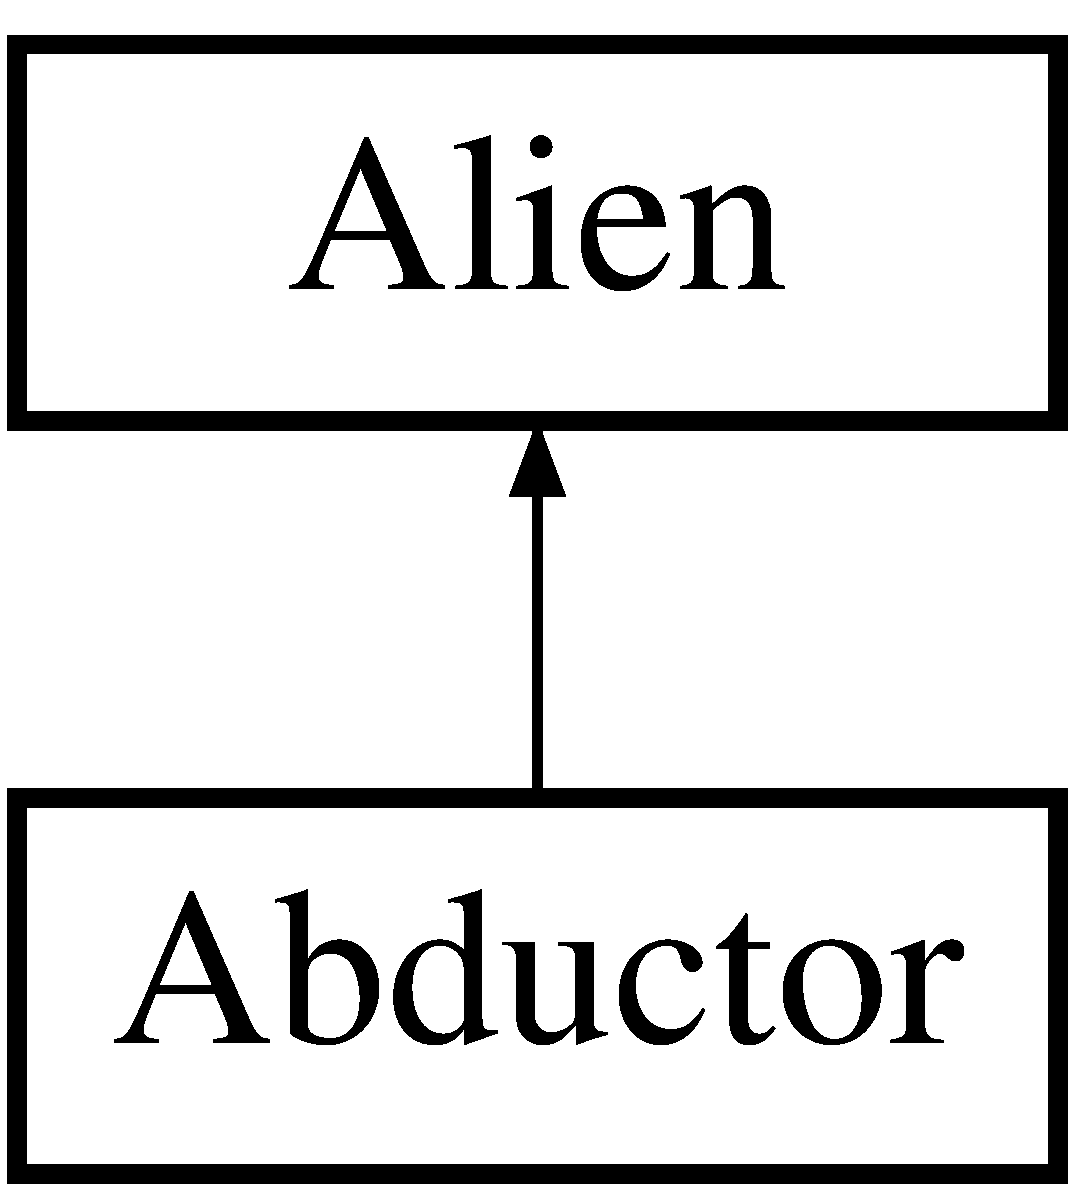
\includegraphics[height=2.000000cm]{class_abductor}
\end{center}
\end{figure}
\subsection*{Public Member Functions}
\begin{DoxyCompactItemize}
\item 
\mbox{\Hypertarget{class_abductor_a0a0e9c59dbef858db23d11c04fb74276}\label{class_abductor_a0a0e9c59dbef858db23d11c04fb74276}} 
\hyperlink{class_abductor_a0a0e9c59dbef858db23d11c04fb74276}{Abductor} (sf\+::\+Vector2f position, float speed, float acceleration)
\begin{DoxyCompactList}\small\item\em \hyperlink{class_abductor}{Abductor} constructor. \end{DoxyCompactList}\item 
void \hyperlink{class_abductor_a0a3080d1631319a1bf890cd0f08935a2}{update} (float dt, \hyperlink{class_alien_manager}{Alien\+Manager} $\ast$data)
\begin{DoxyCompactList}\small\item\em \hyperlink{class_abductor}{Abductor} implementation of \hyperlink{class_alien}{Alien} update. \end{DoxyCompactList}\end{DoxyCompactItemize}
\subsection*{Additional Inherited Members}


\subsection{Detailed Description}
\hyperlink{class_abductor}{Abductor} type alien. 

\hyperlink{class_abductor}{Abductor} type aliens move around in flocks in order to find astronauts. When they find an astronaut they will catch and abduct it, moving slowly towards the top of the screen. If they succeed in abducting an astronaut, the astronaut will become a mutant. Abductors fire single bullets at the player if close enough. 

\subsection{Member Function Documentation}
\mbox{\Hypertarget{class_abductor_a0a3080d1631319a1bf890cd0f08935a2}\label{class_abductor_a0a3080d1631319a1bf890cd0f08935a2}} 
\index{Abductor@{Abductor}!update@{update}}
\index{update@{update}!Abductor@{Abductor}}
\subsubsection{\texorpdfstring{update()}{update()}}
{\footnotesize\ttfamily void Abductor\+::update (\begin{DoxyParamCaption}\item[{float}]{dt,  }\item[{\hyperlink{class_alien_manager}{Alien\+Manager} $\ast$}]{data }\end{DoxyParamCaption})\hspace{0.3cm}{\ttfamily [virtual]}}



\hyperlink{class_abductor}{Abductor} implementation of \hyperlink{class_alien}{Alien} update. 

see \hyperlink{class_alien_afdf9627be2ad37372174a250540dd47b}{Alien\+::update} \hyperlink{class_abductor}{Abductor} behaviour described in class description. 

Implements \hyperlink{class_alien_afdf9627be2ad37372174a250540dd47b}{Alien}.



The documentation for this class was generated from the following files\+:\begin{DoxyCompactItemize}
\item 
A\+I\+Defender\+Project/Abductor.\+h\item 
A\+I\+Defender\+Project/Abductor.\+cpp\end{DoxyCompactItemize}

\hypertarget{class_alien}{}\section{Alien Class Reference}
\label{class_alien}\index{Alien@{Alien}}


\hyperlink{class_alien}{Alien} base class.  




{\ttfamily \#include $<$Alien.\+h$>$}

Inheritance diagram for Alien\+:\begin{figure}[H]
\begin{center}
\leavevmode
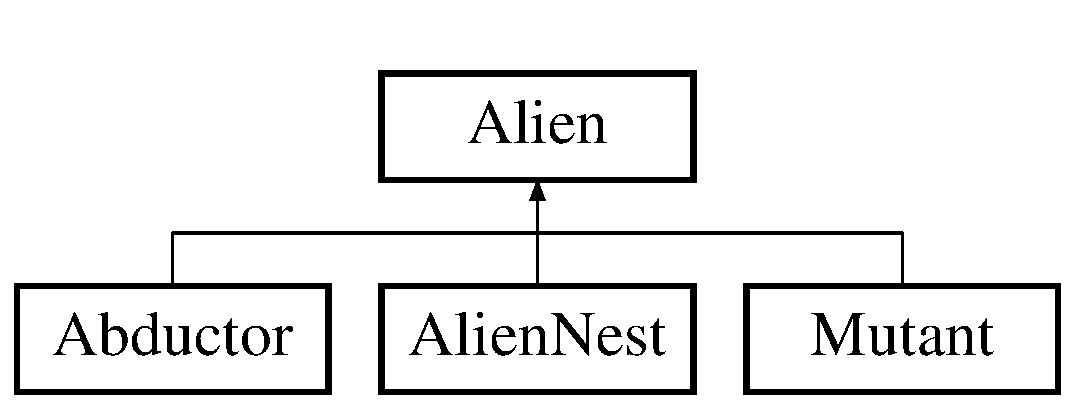
\includegraphics[height=2.000000cm]{class_alien}
\end{center}
\end{figure}
\subsection*{Public Member Functions}
\begin{DoxyCompactItemize}
\item 
\mbox{\Hypertarget{class_alien_a0ac76d63046eed42f2581cb5ec3a493b}\label{class_alien_a0ac76d63046eed42f2581cb5ec3a493b}} 
\hyperlink{class_alien_a0ac76d63046eed42f2581cb5ec3a493b}{Alien} (sf\+::\+Vector2f pos, float speed, float acceleration)
\begin{DoxyCompactList}\small\item\em \hyperlink{class_alien}{Alien} constructor. \end{DoxyCompactList}\item 
virtual void \hyperlink{class_alien_afdf9627be2ad37372174a250540dd47b}{update} (float dt, \hyperlink{class_alien_manager}{Alien\+Manager} $\ast$data)=0
\begin{DoxyCompactList}\small\item\em Unimplemented \hyperlink{class_alien}{Alien} update. \end{DoxyCompactList}\item 
void \hyperlink{class_alien_a8d407e6ec7a582cefe9d7e37b1b3b063}{render} (sf\+::\+Render\+Window $\ast$window, \hyperlink{class_camera}{Camera} $\ast$camera)
\begin{DoxyCompactList}\small\item\em \hyperlink{class_alien}{Alien} render function. \end{DoxyCompactList}\item 
\mbox{\Hypertarget{class_alien_aa9aefdfec02345614bca8ad45779df49}\label{class_alien_aa9aefdfec02345614bca8ad45779df49}} 
sf\+::\+Vector2f \hyperlink{class_alien_aa9aefdfec02345614bca8ad45779df49}{get\+Pos} ()
\begin{DoxyCompactList}\small\item\em returns the \hyperlink{class_alien}{Alien} position \end{DoxyCompactList}\item 
\mbox{\Hypertarget{class_alien_adeddf8c801bcd1c0e18d3bd5323cb287}\label{class_alien_adeddf8c801bcd1c0e18d3bd5323cb287}} 
sf\+::\+Vector2f \hyperlink{class_alien_adeddf8c801bcd1c0e18d3bd5323cb287}{get\+Vel} ()
\begin{DoxyCompactList}\small\item\em returns the \hyperlink{class_alien}{Alien} velocity \end{DoxyCompactList}\item 
\mbox{\Hypertarget{class_alien_a00f66939b33c32f9f5f11f0097b7734b}\label{class_alien_a00f66939b33c32f9f5f11f0097b7734b}} 
sf\+::\+Vector2f \hyperlink{class_alien_a00f66939b33c32f9f5f11f0097b7734b}{get\+Accel} ()
\begin{DoxyCompactList}\small\item\em returns the \hyperlink{class_alien}{Alien} acceleration \end{DoxyCompactList}\item 
\mbox{\Hypertarget{class_alien_afaa2d6ceb2bd11b135b22db941d4a1a1}\label{class_alien_afaa2d6ceb2bd11b135b22db941d4a1a1}} 
Alien\+Type \hyperlink{class_alien_afaa2d6ceb2bd11b135b22db941d4a1a1}{get\+Type} ()
\begin{DoxyCompactList}\small\item\em returns the Type of the \hyperlink{class_alien}{Alien} \end{DoxyCompactList}\end{DoxyCompactItemize}
\subsection*{Protected Member Functions}
\begin{DoxyCompactItemize}
\item 
\mbox{\Hypertarget{class_alien_ae7704be3d9ce25c615bc7ba9ac222432}\label{class_alien_ae7704be3d9ce25c615bc7ba9ac222432}} 
void {\bfseries move} (float dt)
\item 
\mbox{\Hypertarget{class_alien_a0d5a50d82bd051afcd93b0ca14e93739}\label{class_alien_a0d5a50d82bd051afcd93b0ca14e93739}} 
void {\bfseries wander} ()
\item 
\mbox{\Hypertarget{class_alien_aa65980cc0a77a1b346af5ae5b11cba55}\label{class_alien_aa65980cc0a77a1b346af5ae5b11cba55}} 
void {\bfseries avoid\+Bounds} (const \hyperlink{class_terrain}{Terrain} $\ast$terrain)
\end{DoxyCompactItemize}
\subsection*{Protected Attributes}
\begin{DoxyCompactItemize}
\item 
\mbox{\Hypertarget{class_alien_a71049b4775c3bc36f77e9efae7776435}\label{class_alien_a71049b4775c3bc36f77e9efae7776435}} 
const float {\bfseries M\+A\+X\+\_\+\+S\+P\+E\+ED}
\item 
\mbox{\Hypertarget{class_alien_a29f82bd442a48ab652c866e7439e84df}\label{class_alien_a29f82bd442a48ab652c866e7439e84df}} 
const float {\bfseries M\+A\+X\+\_\+\+A\+C\+C\+E\+L\+E\+R\+A\+T\+I\+ON} = 5.\+0f
\item 
\mbox{\Hypertarget{class_alien_a76fc2c3fa215b53ad5aa4b17a763ca3b}\label{class_alien_a76fc2c3fa215b53ad5aa4b17a763ca3b}} 
bool {\bfseries m\+\_\+alive}
\item 
\mbox{\Hypertarget{class_alien_a397e6541d43dde1cdd078aa9d05db811}\label{class_alien_a397e6541d43dde1cdd078aa9d05db811}} 
Alien\+Type {\bfseries m\+\_\+type}
\item 
\mbox{\Hypertarget{class_alien_a8198b0fd2c426e9cc463b61f27951bba}\label{class_alien_a8198b0fd2c426e9cc463b61f27951bba}} 
sf\+::\+Rectangle\+Shape {\bfseries m\+\_\+sprite}
\item 
\mbox{\Hypertarget{class_alien_a322549c43dbbb6bd8ea9200ef3f33cee}\label{class_alien_a322549c43dbbb6bd8ea9200ef3f33cee}} 
sf\+::\+Vector2f {\bfseries m\+\_\+position}
\item 
\mbox{\Hypertarget{class_alien_a7f7f748380d988932e34f5914492c687}\label{class_alien_a7f7f748380d988932e34f5914492c687}} 
sf\+::\+Vector2f {\bfseries m\+\_\+velocity}
\item 
\mbox{\Hypertarget{class_alien_a5eb7b53f9c2d69e3d35fa598f3c083c4}\label{class_alien_a5eb7b53f9c2d69e3d35fa598f3c083c4}} 
sf\+::\+Vector2f {\bfseries m\+\_\+acceleration}
\item 
\mbox{\Hypertarget{class_alien_a46a331850ed1b106efc2541e759ec2bd}\label{class_alien_a46a331850ed1b106efc2541e759ec2bd}} 
float {\bfseries m\+\_\+angle}
\end{DoxyCompactItemize}


\subsection{Detailed Description}
\hyperlink{class_alien}{Alien} base class. 

Pure virtual \hyperlink{class_alien}{Alien} base class for the alien hierarchy tree. Implements the common elements of all aliens and has a pure virtual update function to allow for different \hyperlink{class_alien}{Alien} behaviours. 

\subsection{Member Function Documentation}
\mbox{\Hypertarget{class_alien_a8d407e6ec7a582cefe9d7e37b1b3b063}\label{class_alien_a8d407e6ec7a582cefe9d7e37b1b3b063}} 
\index{Alien@{Alien}!render@{render}}
\index{render@{render}!Alien@{Alien}}
\subsubsection{\texorpdfstring{render()}{render()}}
{\footnotesize\ttfamily void Alien\+::render (\begin{DoxyParamCaption}\item[{sf\+::\+Render\+Window $\ast$}]{window,  }\item[{\hyperlink{class_camera}{Camera} $\ast$}]{camera }\end{DoxyParamCaption})}



\hyperlink{class_alien}{Alien} render function. 


\begin{DoxyParams}{Parameters}
{\em window} & S\+F\+ML window to render to \\
\hline
{\em camera} & adjusts positions based on the camera position draws \hyperlink{class_alien}{Alien} to the screen \\
\hline
\end{DoxyParams}
\mbox{\Hypertarget{class_alien_afdf9627be2ad37372174a250540dd47b}\label{class_alien_afdf9627be2ad37372174a250540dd47b}} 
\index{Alien@{Alien}!update@{update}}
\index{update@{update}!Alien@{Alien}}
\subsubsection{\texorpdfstring{update()}{update()}}
{\footnotesize\ttfamily virtual void Alien\+::update (\begin{DoxyParamCaption}\item[{float}]{dt,  }\item[{\hyperlink{class_alien_manager}{Alien\+Manager} $\ast$}]{data }\end{DoxyParamCaption})\hspace{0.3cm}{\ttfamily [pure virtual]}}



Unimplemented \hyperlink{class_alien}{Alien} update. 


\begin{DoxyParams}{Parameters}
{\em dt} & delta time since last frame \\
\hline
{\em data} & pointer allows abductor access to game data \\
\hline
\end{DoxyParams}


Implemented in \hyperlink{class_abductor_a0a3080d1631319a1bf890cd0f08935a2}{Abductor}, \hyperlink{class_mutant_a38e6f65661b8f81e58f5e06b4d546457}{Mutant}, and \hyperlink{class_alien_nest_ac8d9fe5e35a8a049ae0be1b4f32bd403}{Alien\+Nest}.



The documentation for this class was generated from the following files\+:\begin{DoxyCompactItemize}
\item 
A\+I\+Defender\+Project/Alien.\+h\item 
A\+I\+Defender\+Project/Alien.\+cpp\end{DoxyCompactItemize}

\hypertarget{class_alien_manager}{}\section{Alien\+Manager Class Reference}
\label{class_alien_manager}\index{Alien\+Manager@{Alien\+Manager}}


Manages \hyperlink{class_alien}{Alien} objects.  




{\ttfamily \#include $<$Alien\+Manager.\+h$>$}

\subsection*{Public Member Functions}
\begin{DoxyCompactItemize}
\item 
\hyperlink{class_alien_manager_a742da1e39310d7693fa2fcbc60d7bf15}{Alien\+Manager} (\hyperlink{class_player}{Player} $\ast$player, std\+::vector$<$ \hyperlink{class_astronaut}{Astronaut} $>$ $\ast$astronauts, \hyperlink{class_terrain}{Terrain} $\ast$terrain, \hyperlink{class_camera}{Camera} $\ast$camera)
\begin{DoxyCompactList}\small\item\em \hyperlink{class_alien_manager}{Alien\+Manager} constructor. \end{DoxyCompactList}\item 
\mbox{\Hypertarget{class_alien_manager_a593f0f436f0954d4fc1e432486b746f6}\label{class_alien_manager_a593f0f436f0954d4fc1e432486b746f6}} 
\hyperlink{class_alien_manager_a593f0f436f0954d4fc1e432486b746f6}{$\sim$\+Alien\+Manager} ()
\begin{DoxyCompactList}\small\item\em \hyperlink{class_alien_manager}{Alien\+Manager} destructor. \end{DoxyCompactList}\item 
\mbox{\Hypertarget{class_alien_manager_a0f6713bb3452f5949da43b870ac7b746}\label{class_alien_manager_a0f6713bb3452f5949da43b870ac7b746}} 
const std\+::deque$<$ \hyperlink{class_alien}{Alien} $\ast$ $>$ \hyperlink{class_alien_manager_a0f6713bb3452f5949da43b870ac7b746}{get\+All} () const
\begin{DoxyCompactList}\small\item\em get the \hyperlink{class_alien}{Alien} container \end{DoxyCompactList}\item 
\mbox{\Hypertarget{class_alien_manager_a4af75ee3ee02f8e327d065d1079e37b6}\label{class_alien_manager_a4af75ee3ee02f8e327d065d1079e37b6}} 
std\+::deque$<$ \hyperlink{class_alien}{Alien} $\ast$ $>$\+::iterator \hyperlink{class_alien_manager_a4af75ee3ee02f8e327d065d1079e37b6}{nest\+Begin} ()
\begin{DoxyCompactList}\small\item\em get the start iterator for \hyperlink{class_alien_nest}{Alien\+Nest} \end{DoxyCompactList}\item 
\mbox{\Hypertarget{class_alien_manager_a98744d687508fa936af8fb07189fd599}\label{class_alien_manager_a98744d687508fa936af8fb07189fd599}} 
std\+::deque$<$ \hyperlink{class_alien}{Alien} $\ast$ $>$\+::iterator \hyperlink{class_alien_manager_a98744d687508fa936af8fb07189fd599}{nest\+End} ()
\begin{DoxyCompactList}\small\item\em get the end iterator for \hyperlink{class_alien_nest}{Alien\+Nest} \end{DoxyCompactList}\item 
\mbox{\Hypertarget{class_alien_manager_ae64cfd417be6903c5999281e1ac5a027}\label{class_alien_manager_ae64cfd417be6903c5999281e1ac5a027}} 
std\+::deque$<$ \hyperlink{class_alien}{Alien} $\ast$ $>$\+::iterator \hyperlink{class_alien_manager_ae64cfd417be6903c5999281e1ac5a027}{abductor\+Begin} ()
\begin{DoxyCompactList}\small\item\em get the start iterator for \hyperlink{class_abductor}{Abductor} \end{DoxyCompactList}\item 
\mbox{\Hypertarget{class_alien_manager_a84234e49e21ab00caa9f3f8a492b0b8d}\label{class_alien_manager_a84234e49e21ab00caa9f3f8a492b0b8d}} 
std\+::deque$<$ \hyperlink{class_alien}{Alien} $\ast$ $>$\+::iterator \hyperlink{class_alien_manager_a84234e49e21ab00caa9f3f8a492b0b8d}{abductor\+End} ()
\begin{DoxyCompactList}\small\item\em get the end iterator for \hyperlink{class_abductor}{Abductor} \end{DoxyCompactList}\item 
\mbox{\Hypertarget{class_alien_manager_a9aa20d1193e10765f9a7d52e0729bc29}\label{class_alien_manager_a9aa20d1193e10765f9a7d52e0729bc29}} 
std\+::deque$<$ \hyperlink{class_alien}{Alien} $\ast$ $>$\+::iterator \hyperlink{class_alien_manager_a9aa20d1193e10765f9a7d52e0729bc29}{mutant\+Begin} ()
\begin{DoxyCompactList}\small\item\em get the start iterator for \hyperlink{class_mutant}{Mutant} \end{DoxyCompactList}\item 
\mbox{\Hypertarget{class_alien_manager_ade814cb64a409e7bd2f88be5be159b16}\label{class_alien_manager_ade814cb64a409e7bd2f88be5be159b16}} 
std\+::deque$<$ \hyperlink{class_alien}{Alien} $\ast$ $>$\+::iterator \hyperlink{class_alien_manager_ade814cb64a409e7bd2f88be5be159b16}{mutant\+End} ()
\begin{DoxyCompactList}\small\item\em get the end iterator for \hyperlink{class_mutant}{Mutant} \end{DoxyCompactList}\item 
\mbox{\Hypertarget{class_alien_manager_a0a2ffae7f5a87d94401b0a0375c02dcd}\label{class_alien_manager_a0a2ffae7f5a87d94401b0a0375c02dcd}} 
std\+::vector$<$ \hyperlink{class_astronaut}{Astronaut} $>$ $\ast$ \hyperlink{class_alien_manager_a0a2ffae7f5a87d94401b0a0375c02dcd}{get\+Astronauts} ()
\begin{DoxyCompactList}\small\item\em get the \hyperlink{class_astronaut}{Astronaut} game data \end{DoxyCompactList}\item 
\mbox{\Hypertarget{class_alien_manager_a40c5a7ffc4c38f3c970f63936a87ccd8}\label{class_alien_manager_a40c5a7ffc4c38f3c970f63936a87ccd8}} 
const \hyperlink{class_player}{Player} $\ast$ \hyperlink{class_alien_manager_a40c5a7ffc4c38f3c970f63936a87ccd8}{get\+Player} ()
\begin{DoxyCompactList}\small\item\em get the \hyperlink{class_player}{Player} game data \end{DoxyCompactList}\item 
\mbox{\Hypertarget{class_alien_manager_a5c6478a22609ee2f69a754a3e20c5cc4}\label{class_alien_manager_a5c6478a22609ee2f69a754a3e20c5cc4}} 
const \hyperlink{class_terrain}{Terrain} $\ast$ \hyperlink{class_alien_manager_a5c6478a22609ee2f69a754a3e20c5cc4}{get\+Terrain} ()
\begin{DoxyCompactList}\small\item\em get the \hyperlink{class_terrain}{Terrain} game data \end{DoxyCompactList}\item 
\mbox{\Hypertarget{class_alien_manager_aeaf8bdda166e1db2b0694447e467820c}\label{class_alien_manager_aeaf8bdda166e1db2b0694447e467820c}} 
const \hyperlink{class_camera}{Camera} $\ast$ \hyperlink{class_alien_manager_aeaf8bdda166e1db2b0694447e467820c}{get\+Camera} ()
\begin{DoxyCompactList}\small\item\em get the \hyperlink{class_camera}{Camera} game data \end{DoxyCompactList}\item 
\mbox{\Hypertarget{class_alien_manager_a2a35d52504c40c4e81bdf7212918dbfe}\label{class_alien_manager_a2a35d52504c40c4e81bdf7212918dbfe}} 
void \hyperlink{class_alien_manager_a2a35d52504c40c4e81bdf7212918dbfe}{add\+Nest} (sf\+::\+Vector2f position)
\begin{DoxyCompactList}\small\item\em adds an \hyperlink{class_alien_nest}{Alien\+Nest} to \hyperlink{class_alien}{Alien} container \end{DoxyCompactList}\item 
\mbox{\Hypertarget{class_alien_manager_a5887485929cb6cca8ac030297c4748d1}\label{class_alien_manager_a5887485929cb6cca8ac030297c4748d1}} 
void \hyperlink{class_alien_manager_a5887485929cb6cca8ac030297c4748d1}{add\+Abductor} (sf\+::\+Vector2f position)
\begin{DoxyCompactList}\small\item\em adds an \hyperlink{class_abductor}{Abductor} to \hyperlink{class_alien}{Alien} container \end{DoxyCompactList}\item 
\mbox{\Hypertarget{class_alien_manager_ab7fb2b7a6977ba318f75d6c66acde43b}\label{class_alien_manager_ab7fb2b7a6977ba318f75d6c66acde43b}} 
void \hyperlink{class_alien_manager_ab7fb2b7a6977ba318f75d6c66acde43b}{add\+Mutant} (sf\+::\+Vector2f position)
\begin{DoxyCompactList}\small\item\em adds an \hyperlink{class_mutant}{Mutant} to \hyperlink{class_alien}{Alien} container \end{DoxyCompactList}\item 
void \hyperlink{class_alien_manager_a1ef71e58d02a0cea52eadccdb2b94ad6}{update} (float dt)
\begin{DoxyCompactList}\small\item\em Updates all the \hyperlink{class_alien}{Alien} objects. \end{DoxyCompactList}\item 
void \hyperlink{class_alien_manager_afe738938dd3967a60ee393d956d5e728}{render} (sf\+::\+Render\+Window $\ast$window, \hyperlink{class_camera}{Camera} $\ast$camera)
\begin{DoxyCompactList}\small\item\em Renders all the \hyperlink{class_alien}{Alien} objects. \end{DoxyCompactList}\end{DoxyCompactItemize}


\subsection{Detailed Description}
Manages \hyperlink{class_alien}{Alien} objects. 

Manages the creation, deletion, updating and rendering of all \hyperlink{class_alien}{Alien} objects. Provides an interface to all aliens for other classes. Contains pointers to game data for \hyperlink{class_alien}{Alien} update. 

\subsection{Constructor \& Destructor Documentation}
\mbox{\Hypertarget{class_alien_manager_a742da1e39310d7693fa2fcbc60d7bf15}\label{class_alien_manager_a742da1e39310d7693fa2fcbc60d7bf15}} 
\index{Alien\+Manager@{Alien\+Manager}!Alien\+Manager@{Alien\+Manager}}
\index{Alien\+Manager@{Alien\+Manager}!Alien\+Manager@{Alien\+Manager}}
\subsubsection{\texorpdfstring{Alien\+Manager()}{AlienManager()}}
{\footnotesize\ttfamily Alien\+Manager\+::\+Alien\+Manager (\begin{DoxyParamCaption}\item[{\hyperlink{class_player}{Player} $\ast$}]{player,  }\item[{std\+::vector$<$ \hyperlink{class_astronaut}{Astronaut} $>$ $\ast$}]{astronauts,  }\item[{\hyperlink{class_terrain}{Terrain} $\ast$}]{terrain,  }\item[{\hyperlink{class_camera}{Camera} $\ast$}]{camera }\end{DoxyParamCaption})}



\hyperlink{class_alien_manager}{Alien\+Manager} constructor. 


\begin{DoxyParams}{Parameters}
{\em player} & pointer for \hyperlink{class_player}{Player} game data \\
\hline
{\em astronauts} & pointer for \hyperlink{class_astronaut}{Astronaut} game data \\
\hline
{\em terrain} & pointer for \hyperlink{class_terrain}{Terrain} game data \\
\hline
{\em camera} & pointer for \hyperlink{class_camera}{Camera} game data \\
\hline
\end{DoxyParams}


\subsection{Member Function Documentation}
\mbox{\Hypertarget{class_alien_manager_afe738938dd3967a60ee393d956d5e728}\label{class_alien_manager_afe738938dd3967a60ee393d956d5e728}} 
\index{Alien\+Manager@{Alien\+Manager}!render@{render}}
\index{render@{render}!Alien\+Manager@{Alien\+Manager}}
\subsubsection{\texorpdfstring{render()}{render()}}
{\footnotesize\ttfamily void Alien\+Manager\+::render (\begin{DoxyParamCaption}\item[{sf\+::\+Render\+Window $\ast$}]{window,  }\item[{\hyperlink{class_camera}{Camera} $\ast$}]{camera }\end{DoxyParamCaption})}



Renders all the \hyperlink{class_alien}{Alien} objects. 


\begin{DoxyParams}{Parameters}
{\em window} & S\+F\+ML window to render to \\
\hline
{\em camera} & adjusts positions based on the camera position draws \hyperlink{class_alien}{Alien} to the screen \\
\hline
\end{DoxyParams}
\mbox{\Hypertarget{class_alien_manager_a1ef71e58d02a0cea52eadccdb2b94ad6}\label{class_alien_manager_a1ef71e58d02a0cea52eadccdb2b94ad6}} 
\index{Alien\+Manager@{Alien\+Manager}!update@{update}}
\index{update@{update}!Alien\+Manager@{Alien\+Manager}}
\subsubsection{\texorpdfstring{update()}{update()}}
{\footnotesize\ttfamily void Alien\+Manager\+::update (\begin{DoxyParamCaption}\item[{float}]{dt }\end{DoxyParamCaption})}



Updates all the \hyperlink{class_alien}{Alien} objects. 


\begin{DoxyParams}{Parameters}
{\em dt} & delta time since last frame \\
\hline
\end{DoxyParams}


The documentation for this class was generated from the following files\+:\begin{DoxyCompactItemize}
\item 
A\+I\+Defender\+Project/Alien\+Manager.\+h\item 
A\+I\+Defender\+Project/Alien\+Manager.\+cpp\end{DoxyCompactItemize}

\hypertarget{class_alien_nest}{}\section{Alien\+Nest Class Reference}
\label{class_alien_nest}\index{Alien\+Nest@{Alien\+Nest}}


\hyperlink{class_alien_nest}{Alien\+Nest} type alien.  




{\ttfamily \#include $<$Alien\+Nest.\+h$>$}

Inheritance diagram for Alien\+Nest\+:\begin{figure}[H]
\begin{center}
\leavevmode
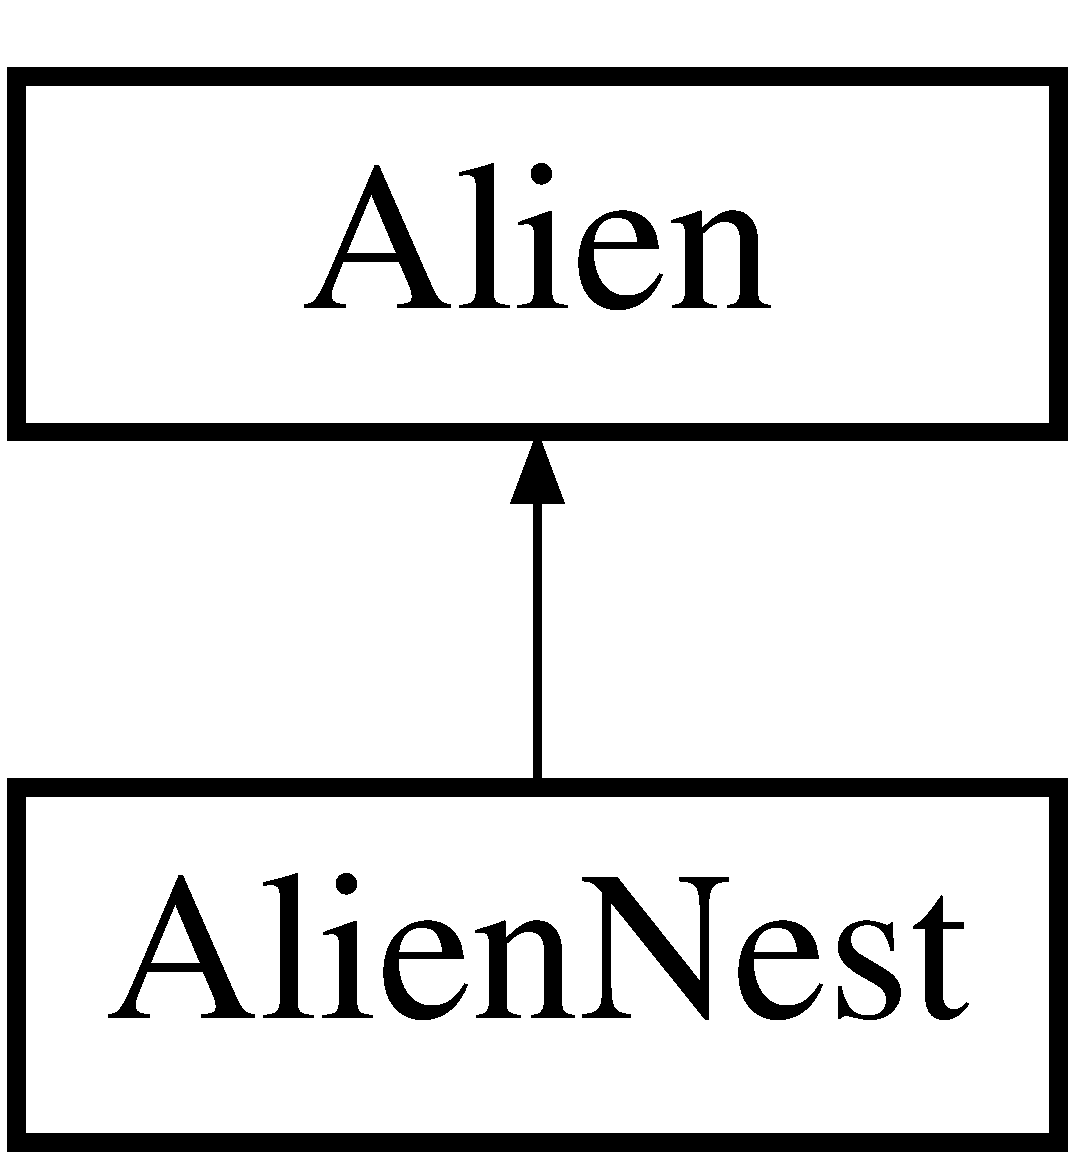
\includegraphics[height=2.000000cm]{class_alien_nest}
\end{center}
\end{figure}
\subsection*{Public Member Functions}
\begin{DoxyCompactItemize}
\item 
\mbox{\Hypertarget{class_alien_nest_ad40eb25b1de5f065ef7d3cdd601847cb}\label{class_alien_nest_ad40eb25b1de5f065ef7d3cdd601847cb}} 
\hyperlink{class_alien_nest_ad40eb25b1de5f065ef7d3cdd601847cb}{Alien\+Nest} (sf\+::\+Vector2f position, float speed, float acceleration)
\begin{DoxyCompactList}\small\item\em \hyperlink{class_alien_nest}{Alien\+Nest} constructor. \end{DoxyCompactList}\item 
void \hyperlink{class_alien_nest_ac8d9fe5e35a8a049ae0be1b4f32bd403}{update} (float dt, \hyperlink{class_alien_manager}{Alien\+Manager} $\ast$data)
\begin{DoxyCompactList}\small\item\em \hyperlink{class_alien_nest}{Alien\+Nest} implementation of \hyperlink{class_alien}{Alien} update. \end{DoxyCompactList}\end{DoxyCompactItemize}
\subsection*{Additional Inherited Members}


\subsection{Detailed Description}
\hyperlink{class_alien_nest}{Alien\+Nest} type alien. 

\hyperlink{class_alien_nest}{Alien\+Nest} type aliens avoid the player, firing guided missiles if they stray too close. Other than that these aliens simply wander and spawn abductors at random intervals. 

\subsection{Member Function Documentation}
\mbox{\Hypertarget{class_alien_nest_ac8d9fe5e35a8a049ae0be1b4f32bd403}\label{class_alien_nest_ac8d9fe5e35a8a049ae0be1b4f32bd403}} 
\index{Alien\+Nest@{Alien\+Nest}!update@{update}}
\index{update@{update}!Alien\+Nest@{Alien\+Nest}}
\subsubsection{\texorpdfstring{update()}{update()}}
{\footnotesize\ttfamily void Alien\+Nest\+::update (\begin{DoxyParamCaption}\item[{float}]{dt,  }\item[{\hyperlink{class_alien_manager}{Alien\+Manager} $\ast$}]{data }\end{DoxyParamCaption})\hspace{0.3cm}{\ttfamily [virtual]}}



\hyperlink{class_alien_nest}{Alien\+Nest} implementation of \hyperlink{class_alien}{Alien} update. 

see \hyperlink{class_alien_afdf9627be2ad37372174a250540dd47b}{Alien\+::update} \hyperlink{class_alien_nest}{Alien\+Nest} behaviour described in class description. 

Implements \hyperlink{class_alien_afdf9627be2ad37372174a250540dd47b}{Alien}.



The documentation for this class was generated from the following files\+:\begin{DoxyCompactItemize}
\item 
A\+I\+Defender\+Project/Alien\+Nest.\+h\item 
A\+I\+Defender\+Project/Alien\+Nest.\+cpp\end{DoxyCompactItemize}

\hypertarget{class_astronaut}{}\section{Astronaut Class Reference}
\label{class_astronaut}\index{Astronaut@{Astronaut}}
\subsection*{Public Member Functions}
\begin{DoxyCompactItemize}
\item 
\mbox{\Hypertarget{class_astronaut_a614b65279635ce7d565fd38d7f8a23a9}\label{class_astronaut_a614b65279635ce7d565fd38d7f8a23a9}} 
{\bfseries Astronaut} (float x=0, \hyperlink{class_alien_manager}{Alien\+Manager} $\ast$alien\+Manager=nullptr)
\item 
\mbox{\Hypertarget{class_astronaut_a4f11ba0fed0d53f93e8c8298bed274bd}\label{class_astronaut_a4f11ba0fed0d53f93e8c8298bed274bd}} 
void {\bfseries update} (float dt, \hyperlink{class_terrain}{Terrain} $\ast$terrain)
\item 
\mbox{\Hypertarget{class_astronaut_aac035dcb12e48dd073057fb84e9b838e}\label{class_astronaut_aac035dcb12e48dd073057fb84e9b838e}} 
void {\bfseries render} (sf\+::\+Render\+Window $\ast$window, \hyperlink{class_camera}{Camera} $\ast$camera)
\item 
\mbox{\Hypertarget{class_astronaut_a86023466ed8a021f668c68fc10f778b0}\label{class_astronaut_a86023466ed8a021f668c68fc10f778b0}} 
void {\bfseries avoid} ()
\item 
\mbox{\Hypertarget{class_astronaut_a39d7e43f8604bf561570e2eb2564a8fa}\label{class_astronaut_a39d7e43f8604bf561570e2eb2564a8fa}} 
void {\bfseries wander} ()
\item 
\mbox{\Hypertarget{class_astronaut_a1699b7aa32a145afbf52166453a4978f}\label{class_astronaut_a1699b7aa32a145afbf52166453a4978f}} 
bool {\bfseries is\+Alien\+Near} ()
\item 
\mbox{\Hypertarget{class_astronaut_a0ff0404afaa68a7f997f06c2b31da64d}\label{class_astronaut_a0ff0404afaa68a7f997f06c2b31da64d}} 
sf\+::\+Vector2f {\bfseries get\+Pos} () const
\item 
\mbox{\Hypertarget{class_astronaut_a846e03bbd9c74739f9943fcccc9c9256}\label{class_astronaut_a846e03bbd9c74739f9943fcccc9c9256}} 
bool {\bfseries get\+Alive} () const
\item 
\mbox{\Hypertarget{class_astronaut_a958f10e0ab8eaacd9317012c6b0a7cba}\label{class_astronaut_a958f10e0ab8eaacd9317012c6b0a7cba}} 
void {\bfseries set\+Pos} (sf\+::\+Vector2f val)
\item 
\mbox{\Hypertarget{class_astronaut_a383b5caca9e2d81a987211eeffec2962}\label{class_astronaut_a383b5caca9e2d81a987211eeffec2962}} 
void {\bfseries set\+Being\+Abducted} (bool val)
\item 
\mbox{\Hypertarget{class_astronaut_aed00a217278aeec62252b906f87a4bd0}\label{class_astronaut_aed00a217278aeec62252b906f87a4bd0}} 
void {\bfseries set\+Alive} (bool val)
\end{DoxyCompactItemize}


The documentation for this class was generated from the following files\+:\begin{DoxyCompactItemize}
\item 
A\+I\+Defender\+Project/Astronaut.\+h\item 
A\+I\+Defender\+Project/Astronaut.\+cpp\end{DoxyCompactItemize}

\hypertarget{class_bullet}{}\section{Bullet Class Reference}
\label{class_bullet}\index{Bullet@{Bullet}}
Inheritance diagram for Bullet\+:\begin{figure}[H]
\begin{center}
\leavevmode
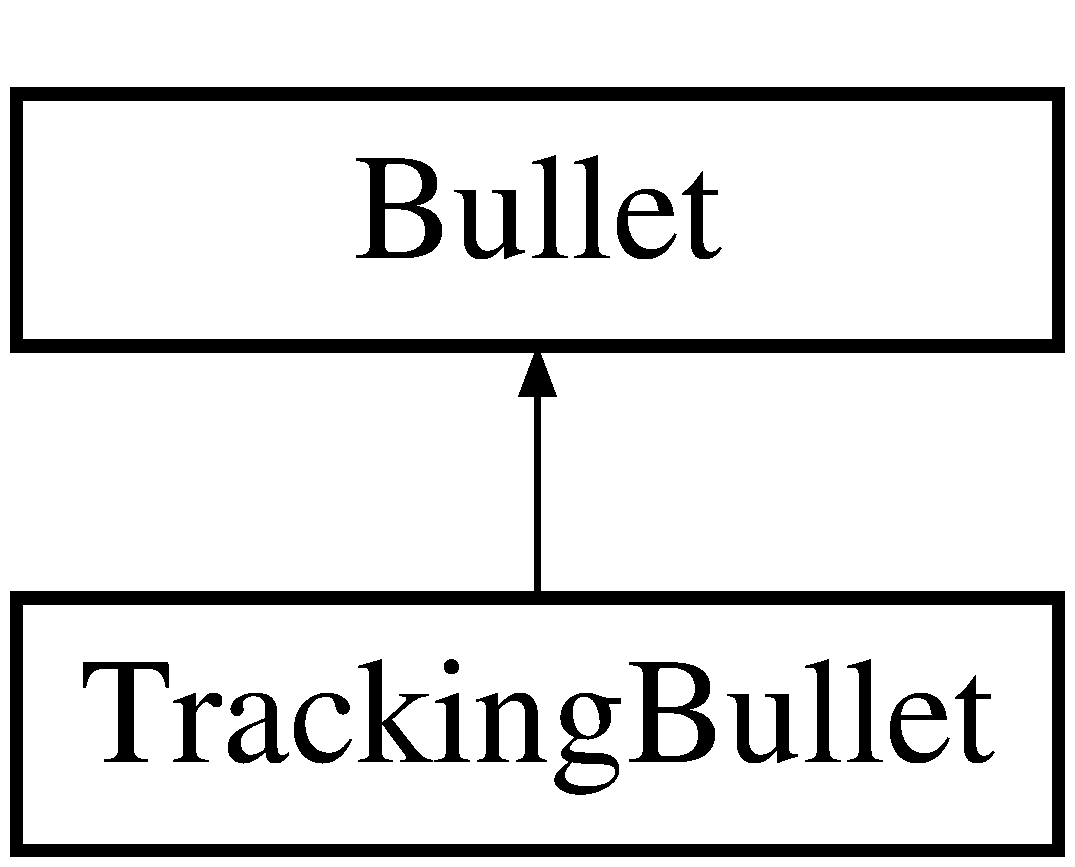
\includegraphics[height=2.000000cm]{class_bullet}
\end{center}
\end{figure}
\subsection*{Public Member Functions}
\begin{DoxyCompactItemize}
\item 
\mbox{\Hypertarget{class_bullet_a77d3b716065155100cb36b354d946cfa}\label{class_bullet_a77d3b716065155100cb36b354d946cfa}} 
{\bfseries Bullet} (sf\+::\+Vector2f, sf\+::\+Vector2f, bool)
\item 
\mbox{\Hypertarget{class_bullet_a32f4a0611fe2dd245fee955d14ca1f68}\label{class_bullet_a32f4a0611fe2dd245fee955d14ca1f68}} 
void {\bfseries update} ()
\item 
\mbox{\Hypertarget{class_bullet_a76ff2859d498ae4f04185bde59139761}\label{class_bullet_a76ff2859d498ae4f04185bde59139761}} 
sf\+::\+Vector2f {\bfseries Normalize} (sf\+::\+Vector2f)
\item 
\mbox{\Hypertarget{class_bullet_ae10a23ad456a1c093ff5ac284776fbaa}\label{class_bullet_ae10a23ad456a1c093ff5ac284776fbaa}} 
void {\bfseries render} (sf\+::\+Render\+Window $\ast$window, \hyperlink{class_camera}{Camera} $\ast$camera)
\item 
\mbox{\Hypertarget{class_bullet_a4c8a3cbe18fadf1c5ed5f2a4322f311a}\label{class_bullet_a4c8a3cbe18fadf1c5ed5f2a4322f311a}} 
void {\bfseries reset} (sf\+::\+Vector2f, sf\+::\+Vector2f, bool)
\item 
\mbox{\Hypertarget{class_bullet_a75b9dbc9c7dc5f0dda65759bc895ac10}\label{class_bullet_a75b9dbc9c7dc5f0dda65759bc895ac10}} 
bool {\bfseries get\+Alive} ()
\item 
\mbox{\Hypertarget{class_bullet_a9553313fc54ced53b8f0952f519c0d8d}\label{class_bullet_a9553313fc54ced53b8f0952f519c0d8d}} 
bool {\bfseries get\+Is\+Enemy\+Bullet} ()
\item 
\mbox{\Hypertarget{class_bullet_aa0163d91e28a47cd89cfdda4923bd30a}\label{class_bullet_aa0163d91e28a47cd89cfdda4923bd30a}} 
sf\+::\+Vector2f {\bfseries get\+Pos} ()
\end{DoxyCompactItemize}
\subsection*{Protected Attributes}
\begin{DoxyCompactItemize}
\item 
\mbox{\Hypertarget{class_bullet_ab7413a852b4a61d3afa739915f6aabee}\label{class_bullet_ab7413a852b4a61d3afa739915f6aabee}} 
sf\+::\+Time {\bfseries life\+Span} = sf\+::seconds(4.\+0f)
\item 
\mbox{\Hypertarget{class_bullet_ae4fd7b85677ea372cab42e70e41cc912}\label{class_bullet_ae4fd7b85677ea372cab42e70e41cc912}} 
sf\+::\+Vector2f {\bfseries m\+\_\+pos}
\item 
\mbox{\Hypertarget{class_bullet_a0fbc2ea9fe4168f68919287ae4243775}\label{class_bullet_a0fbc2ea9fe4168f68919287ae4243775}} 
sf\+::\+Vector2f {\bfseries m\+\_\+vel}
\item 
\mbox{\Hypertarget{class_bullet_aea01c8f427c24c577bb2a481c8e42d44}\label{class_bullet_aea01c8f427c24c577bb2a481c8e42d44}} 
sf\+::\+Clock {\bfseries m\+\_\+clock}
\item 
\mbox{\Hypertarget{class_bullet_a82d28a9015bb71d7ab456be754388963}\label{class_bullet_a82d28a9015bb71d7ab456be754388963}} 
sf\+::\+Time {\bfseries m\+\_\+start\+Time}
\item 
\mbox{\Hypertarget{class_bullet_a7a3ba271067cbba6decf7adfa0583b07}\label{class_bullet_a7a3ba271067cbba6decf7adfa0583b07}} 
sf\+::\+Circle\+Shape {\bfseries m\+\_\+sprite}
\item 
\mbox{\Hypertarget{class_bullet_a81722b39f1333ae333103844bb827f5d}\label{class_bullet_a81722b39f1333ae333103844bb827f5d}} 
bool {\bfseries m\+\_\+alive}
\item 
\mbox{\Hypertarget{class_bullet_aa831ee51deecd215702614f4232b97e5}\label{class_bullet_aa831ee51deecd215702614f4232b97e5}} 
bool {\bfseries m\+\_\+is\+Enemy\+Bullet}
\end{DoxyCompactItemize}


The documentation for this class was generated from the following files\+:\begin{DoxyCompactItemize}
\item 
A\+I\+Defender\+Project/Bullet.\+h\item 
A\+I\+Defender\+Project/Bullet.\+cpp\end{DoxyCompactItemize}

\hypertarget{class_bullet_manager}{}\section{Bullet\+Manager Class Reference}
\label{class_bullet_manager}\index{Bullet\+Manager@{Bullet\+Manager}}
\subsection*{Public Member Functions}
\begin{DoxyCompactItemize}
\item 
\mbox{\Hypertarget{class_bullet_manager_a7033a1eceb09644c8d0084c9d34c7b43}\label{class_bullet_manager_a7033a1eceb09644c8d0084c9d34c7b43}} 
void {\bfseries add\+Bullet} (sf\+::\+Vector2f, sf\+::\+Vector2f, bool, bool)
\item 
\mbox{\Hypertarget{class_bullet_manager_ae8638f3b70fe44a15413e1107ea806fe}\label{class_bullet_manager_ae8638f3b70fe44a15413e1107ea806fe}} 
void {\bfseries update} ()
\item 
\mbox{\Hypertarget{class_bullet_manager_a42da1416dcbc47691ee6722eb8b744c1}\label{class_bullet_manager_a42da1416dcbc47691ee6722eb8b744c1}} 
bool {\bfseries check\+Collision} (int, sf\+::\+Rectangle\+Shape)
\item 
\mbox{\Hypertarget{class_bullet_manager_afbb0727bcda4c29055c23604fb60536b}\label{class_bullet_manager_afbb0727bcda4c29055c23604fb60536b}} 
void {\bfseries render} (sf\+::\+Render\+Window $\ast$window, \hyperlink{class_camera}{Camera} $\ast$camera)
\item 
\mbox{\Hypertarget{class_bullet_manager_a923c9563f241934310838bbbb7864dda}\label{class_bullet_manager_a923c9563f241934310838bbbb7864dda}} 
bool {\bfseries get\+Is\+Enemy\+Bullet} (int index)
\end{DoxyCompactItemize}
\subsection*{Static Public Member Functions}
\begin{DoxyCompactItemize}
\item 
\mbox{\Hypertarget{class_bullet_manager_a64c2602d2431ffe986b789bfc4f8e729}\label{class_bullet_manager_a64c2602d2431ffe986b789bfc4f8e729}} 
static \hyperlink{class_bullet_manager}{Bullet\+Manager} $\ast$ {\bfseries get\+Instance} ()
\end{DoxyCompactItemize}


The documentation for this class was generated from the following files\+:\begin{DoxyCompactItemize}
\item 
A\+I\+Defender\+Project/Bullet\+Manager.\+h\item 
A\+I\+Defender\+Project/Bullet\+Manager.\+cpp\end{DoxyCompactItemize}

\hypertarget{class_camera}{}\section{Camera Class Reference}
\label{class_camera}\index{Camera@{Camera}}
\subsection*{Public Member Functions}
\begin{DoxyCompactItemize}
\item 
\mbox{\Hypertarget{class_camera_a7827bfde3038e43f3ee29dc2173f90d1}\label{class_camera_a7827bfde3038e43f3ee29dc2173f90d1}} 
{\bfseries Camera} (int screen\+Width=0, int screen\+Height=0, int world\+Width=0, int world\+Height=0)
\item 
\mbox{\Hypertarget{class_camera_a1336e459c3ff1ea383546d12ddbae790}\label{class_camera_a1336e459c3ff1ea383546d12ddbae790}} 
void {\bfseries update} (sf\+::\+Vector2f centre)
\item 
\mbox{\Hypertarget{class_camera_a48842371f914137c7c5311789789633a}\label{class_camera_a48842371f914137c7c5311789789633a}} 
sf\+::\+Vector2f {\bfseries operator+} (sf\+::\+Vector2f vec) const
\item 
\mbox{\Hypertarget{class_camera_a5ad7481d9f6ca0c3374cddb2ba3d1ea8}\label{class_camera_a5ad7481d9f6ca0c3374cddb2ba3d1ea8}} 
sf\+::\+Sprite {\bfseries operator+} (sf\+::\+Sprite spr)
\end{DoxyCompactItemize}


The documentation for this class was generated from the following files\+:\begin{DoxyCompactItemize}
\item 
A\+I\+Defender\+Project/Camera.\+h\item 
A\+I\+Defender\+Project/Camera.\+cpp\end{DoxyCompactItemize}

\hypertarget{class_event_listener}{}\section{Event\+Listener Class Reference}
\label{class_event_listener}\index{Event\+Listener@{Event\+Listener}}
Inheritance diagram for Event\+Listener\+:\begin{figure}[H]
\begin{center}
\leavevmode
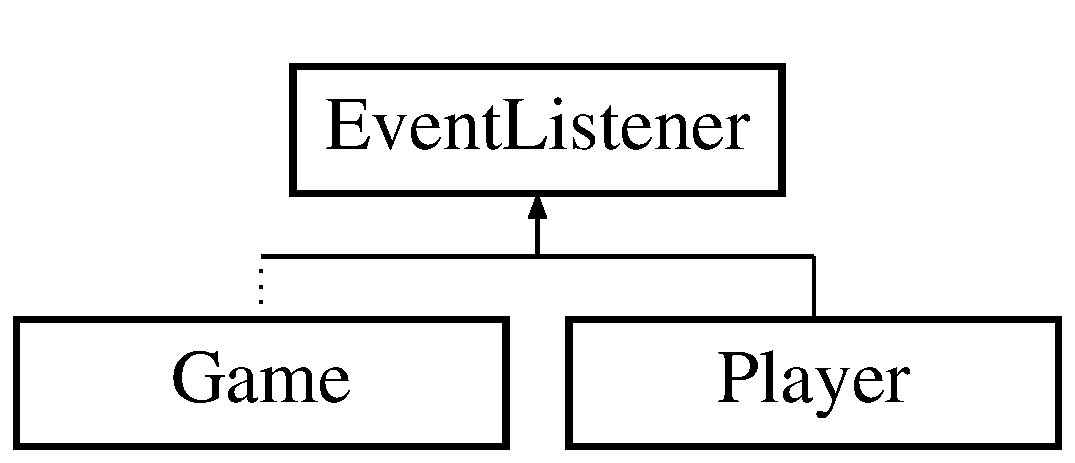
\includegraphics[height=2.000000cm]{class_event_listener}
\end{center}
\end{figure}
\subsection*{Public Member Functions}
\begin{DoxyCompactItemize}
\item 
\mbox{\Hypertarget{class_event_listener_a9c9605986d289a8ad888540a21339cf4}\label{class_event_listener_a9c9605986d289a8ad888540a21339cf4}} 
virtual void {\bfseries on\+Event} (sf\+::\+Event)=0
\end{DoxyCompactItemize}


The documentation for this class was generated from the following file\+:\begin{DoxyCompactItemize}
\item 
A\+I\+Defender\+Project/Event\+Listener.\+h\end{DoxyCompactItemize}

\hypertarget{class_game}{}\section{Game Class Reference}
\label{class_game}\index{Game@{Game}}


Class manages game logic.  




{\ttfamily \#include $<$Game.\+h$>$}

Inheritance diagram for Game\+:\begin{figure}[H]
\begin{center}
\leavevmode
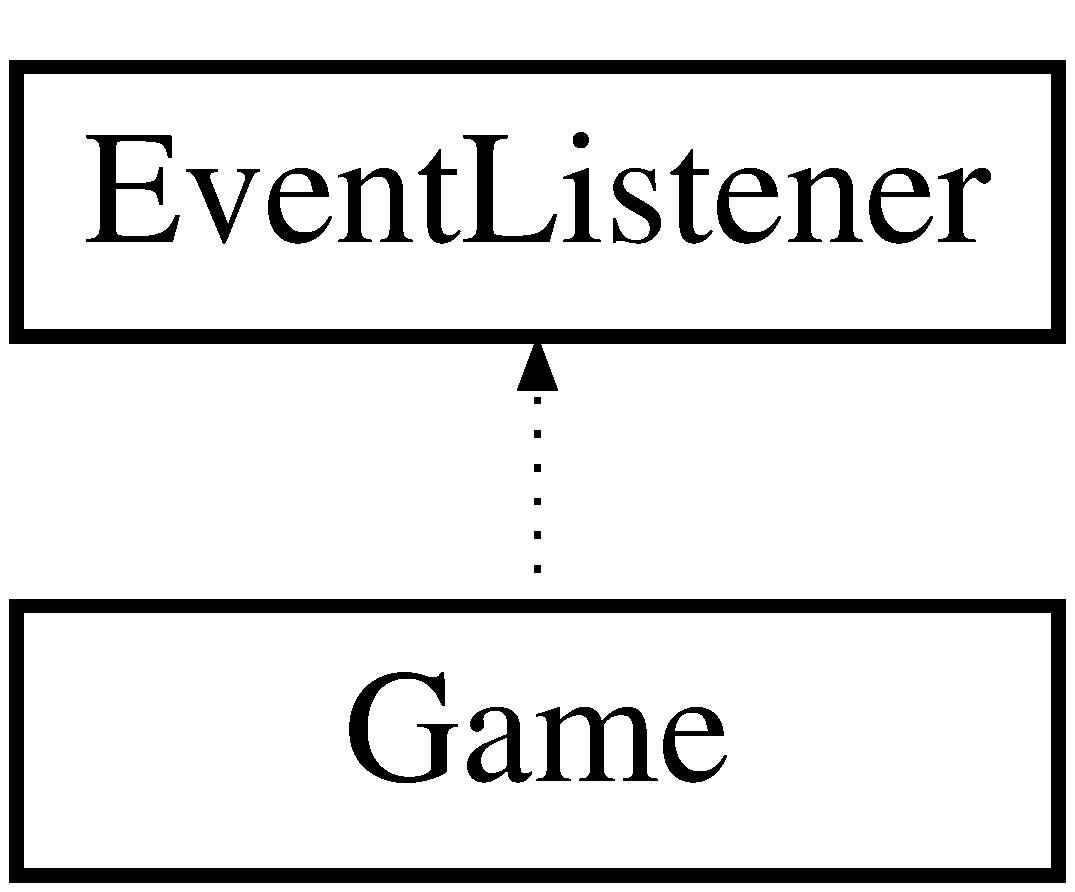
\includegraphics[height=2.000000cm]{class_game}
\end{center}
\end{figure}
\subsection*{Public Member Functions}
\begin{DoxyCompactItemize}
\item 
\mbox{\Hypertarget{class_game_ad59df6562a58a614fda24622d3715b65}\label{class_game_ad59df6562a58a614fda24622d3715b65}} 
\hyperlink{class_game_ad59df6562a58a614fda24622d3715b65}{Game} ()
\begin{DoxyCompactList}\small\item\em \hyperlink{class_game}{Game} constructor. \end{DoxyCompactList}\item 
\mbox{\Hypertarget{class_game_a7ad92b77b596d7882a7ae76eb18b5e6c}\label{class_game_a7ad92b77b596d7882a7ae76eb18b5e6c}} 
void \hyperlink{class_game_a7ad92b77b596d7882a7ae76eb18b5e6c}{loop} ()
\begin{DoxyCompactList}\small\item\em \hyperlink{class_game}{Game} loop, all run time game logic executed here. \end{DoxyCompactList}\item 
\mbox{\Hypertarget{class_game_a9f1e6b43d3f4136d7293c3bfc852770b}\label{class_game_a9f1e6b43d3f4136d7293c3bfc852770b}} 
void \hyperlink{class_game_a9f1e6b43d3f4136d7293c3bfc852770b}{on\+Event} (sf\+::\+Event evt)
\begin{DoxyCompactList}\small\item\em \hyperlink{class_game}{Game} responds to key events here. \end{DoxyCompactList}\end{DoxyCompactItemize}


\subsection{Detailed Description}
Class manages game logic. 

This class includes all the game logic and is the controller class for the project. It contains all the game entities and manages communication between them. 

The documentation for this class was generated from the following files\+:\begin{DoxyCompactItemize}
\item 
A\+I\+Defender\+Project/Game.\+h\item 
A\+I\+Defender\+Project/Game.\+cpp\end{DoxyCompactItemize}

\hypertarget{class_input_manager}{}\section{Input\+Manager Class Reference}
\label{class_input_manager}\index{Input\+Manager@{Input\+Manager}}
\subsection*{Public Member Functions}
\begin{DoxyCompactItemize}
\item 
\mbox{\Hypertarget{class_input_manager_a425a05f7defe636300aa67f31ba8e69a}\label{class_input_manager_a425a05f7defe636300aa67f31ba8e69a}} 
{\bfseries Input\+Manager} (sf\+::\+Window $\ast$window=nullptr)
\item 
\mbox{\Hypertarget{class_input_manager_a45002a46e5bdcb505d5c6a63987333bd}\label{class_input_manager_a45002a46e5bdcb505d5c6a63987333bd}} 
void {\bfseries add\+Listener} (sf\+::\+Event\+::\+Event\+Type, \hyperlink{class_event_listener}{Event\+Listener} $\ast$)
\item 
\mbox{\Hypertarget{class_input_manager_aed7568fce1d9e66f3e98032de3b51c16}\label{class_input_manager_aed7568fce1d9e66f3e98032de3b51c16}} 
void {\bfseries add\+Callback} (sf\+::\+Event\+::\+Event\+Type, void($\ast$func)(sf\+::\+Event))
\item 
\mbox{\Hypertarget{class_input_manager_a5cf3293b1e67db618284ff0040c0ddff}\label{class_input_manager_a5cf3293b1e67db618284ff0040c0ddff}} 
void {\bfseries dispatch} (sf\+::\+Event)
\item 
\mbox{\Hypertarget{class_input_manager_a5a14083a10c5d2da3febe3f6e68f6803}\label{class_input_manager_a5a14083a10c5d2da3febe3f6e68f6803}} 
void {\bfseries process\+Input} ()
\end{DoxyCompactItemize}


The documentation for this class was generated from the following files\+:\begin{DoxyCompactItemize}
\item 
A\+I\+Defender\+Project/Input\+Manager.\+h\item 
A\+I\+Defender\+Project/Input\+Manager.\+cpp\end{DoxyCompactItemize}

\hypertarget{class_mutant}{}\section{Mutant Class Reference}
\label{class_mutant}\index{Mutant@{Mutant}}


\hyperlink{class_mutant}{Mutant} type alien.  




{\ttfamily \#include $<$Mutant.\+h$>$}

Inheritance diagram for Mutant\+:\begin{figure}[H]
\begin{center}
\leavevmode
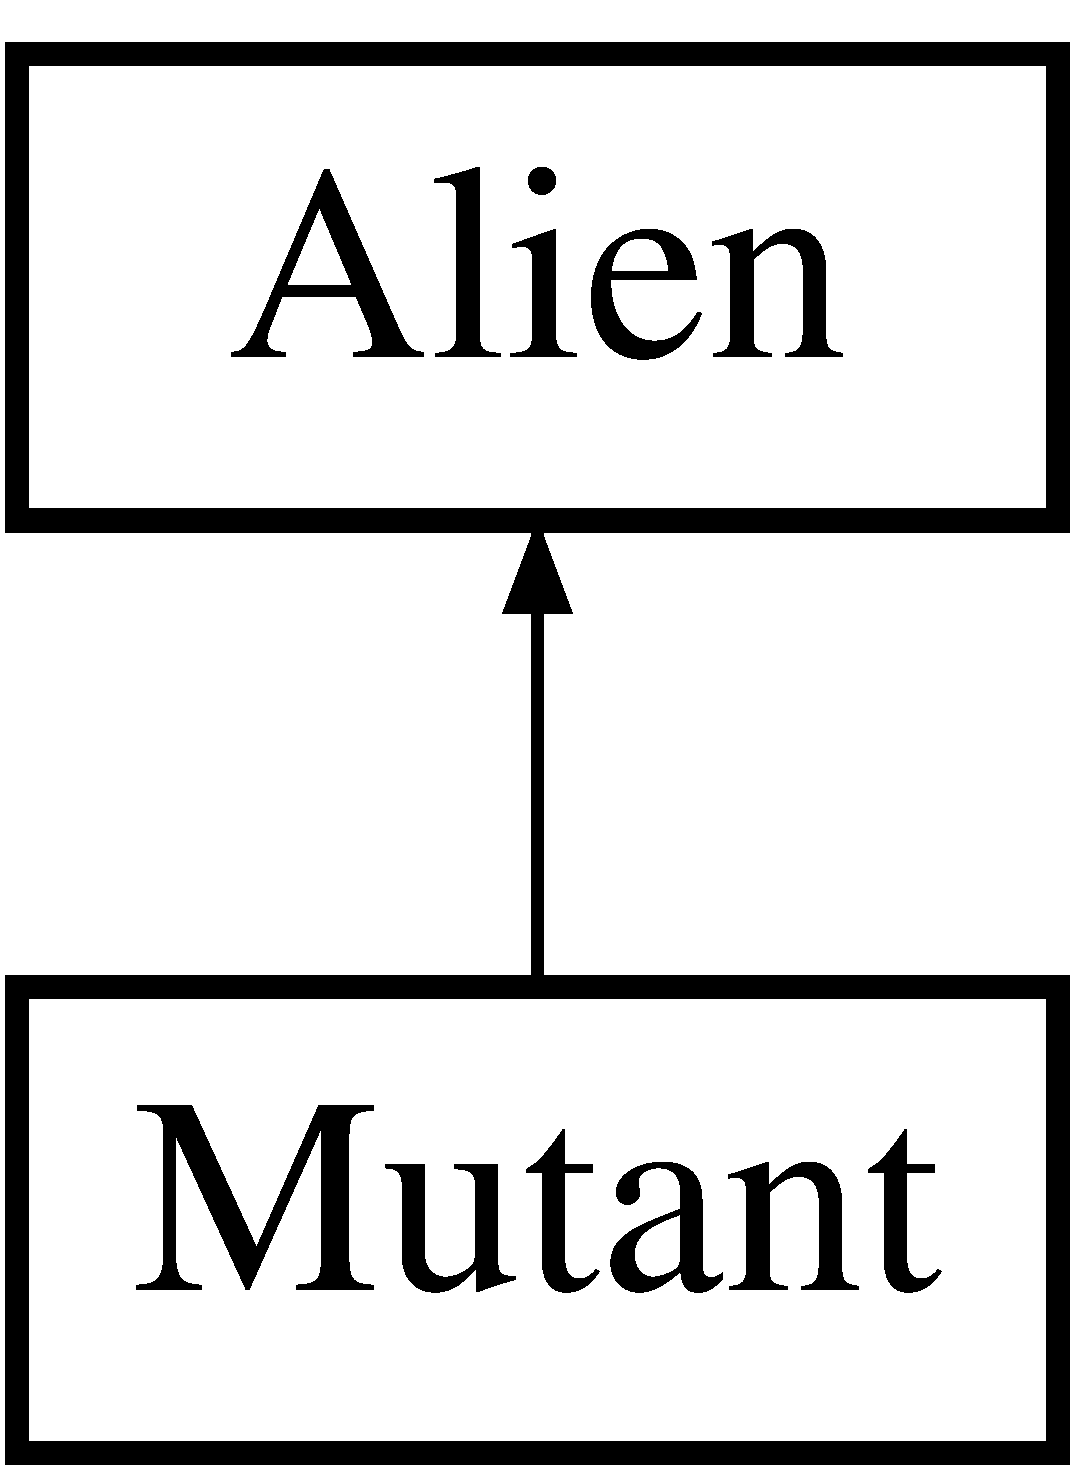
\includegraphics[height=2.000000cm]{class_mutant}
\end{center}
\end{figure}
\subsection*{Public Member Functions}
\begin{DoxyCompactItemize}
\item 
\mbox{\Hypertarget{class_mutant_ab0050fd2b81983b932404a0f83289198}\label{class_mutant_ab0050fd2b81983b932404a0f83289198}} 
\hyperlink{class_mutant_ab0050fd2b81983b932404a0f83289198}{Mutant} (sf\+::\+Vector2f position, float speed, float acceleration)
\begin{DoxyCompactList}\small\item\em \hyperlink{class_mutant}{Mutant} constructor. \end{DoxyCompactList}\item 
void \hyperlink{class_mutant_a38e6f65661b8f81e58f5e06b4d546457}{update} (float dt, \hyperlink{class_alien_manager}{Alien\+Manager} $\ast$data)
\begin{DoxyCompactList}\small\item\em \hyperlink{class_mutant}{Mutant} implementation of \hyperlink{class_alien}{Alien} update. \end{DoxyCompactList}\end{DoxyCompactItemize}
\subsection*{Additional Inherited Members}


\subsection{Detailed Description}
\hyperlink{class_mutant}{Mutant} type alien. 

\hyperlink{class_mutant}{Mutant} type aliens collect into swarms. They aggresively seek the player and will attack the player using some intelligent behaviours. 

\subsection{Member Function Documentation}
\mbox{\Hypertarget{class_mutant_a38e6f65661b8f81e58f5e06b4d546457}\label{class_mutant_a38e6f65661b8f81e58f5e06b4d546457}} 
\index{Mutant@{Mutant}!update@{update}}
\index{update@{update}!Mutant@{Mutant}}
\subsubsection{\texorpdfstring{update()}{update()}}
{\footnotesize\ttfamily void Mutant\+::update (\begin{DoxyParamCaption}\item[{float}]{dt,  }\item[{\hyperlink{class_alien_manager}{Alien\+Manager} $\ast$}]{data }\end{DoxyParamCaption})\hspace{0.3cm}{\ttfamily [virtual]}}



\hyperlink{class_mutant}{Mutant} implementation of \hyperlink{class_alien}{Alien} update. 

see \hyperlink{class_alien_afdf9627be2ad37372174a250540dd47b}{Alien\+::update} \hyperlink{class_mutant}{Mutant} behaviour described in class description. 

Implements \hyperlink{class_alien_afdf9627be2ad37372174a250540dd47b}{Alien}.



The documentation for this class was generated from the following files\+:\begin{DoxyCompactItemize}
\item 
A\+I\+Defender\+Project/Mutant.\+h\item 
A\+I\+Defender\+Project/Mutant.\+cpp\end{DoxyCompactItemize}

\hypertarget{class_player}{}\section{Player Class Reference}
\label{class_player}\index{Player@{Player}}
Inheritance diagram for Player\+:\begin{figure}[H]
\begin{center}
\leavevmode
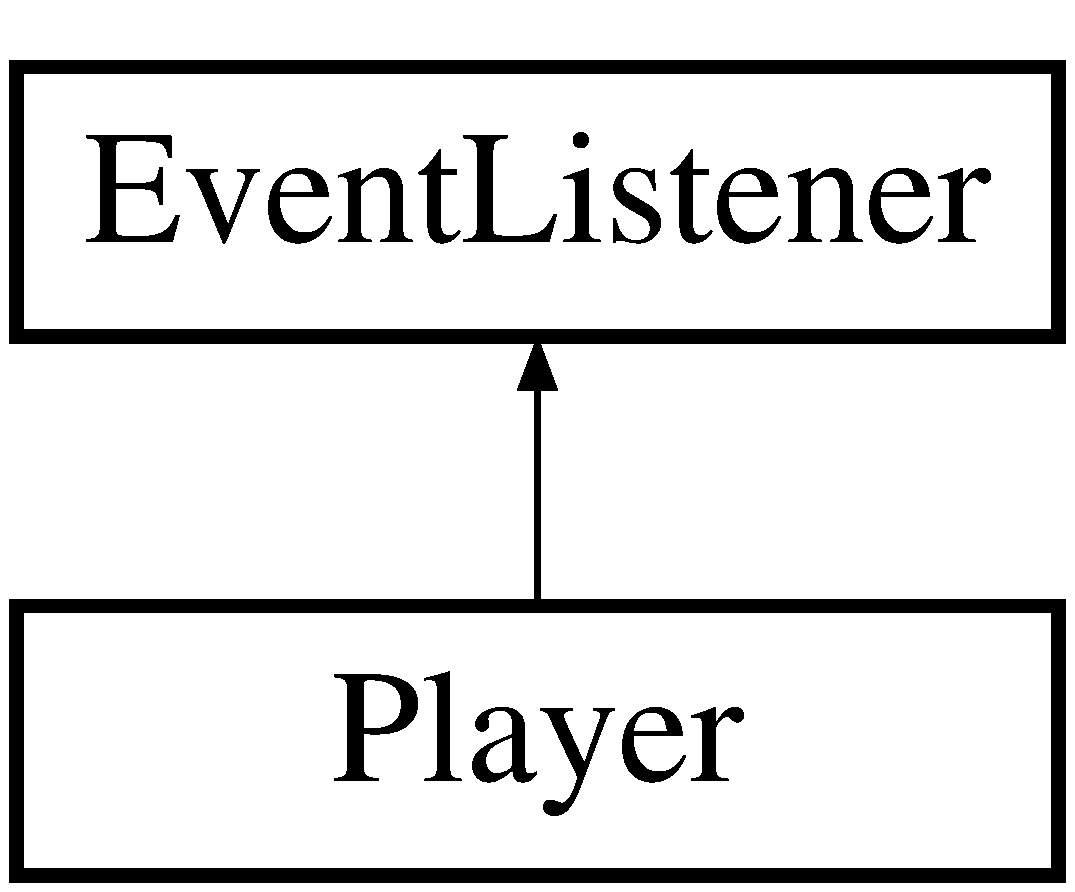
\includegraphics[height=2.000000cm]{class_player}
\end{center}
\end{figure}
\subsection*{Public Member Functions}
\begin{DoxyCompactItemize}
\item 
\mbox{\Hypertarget{class_player_ae7812e67381f4c26ae1b963eeaffc3a1}\label{class_player_ae7812e67381f4c26ae1b963eeaffc3a1}} 
void {\bfseries update} (float dt)
\item 
\mbox{\Hypertarget{class_player_afc1d17f6c3dd5538f50fcc4b6474045e}\label{class_player_afc1d17f6c3dd5538f50fcc4b6474045e}} 
void {\bfseries render} (sf\+::\+Render\+Window $\ast$window, \hyperlink{class_camera}{Camera} $\ast$camera)
\item 
\mbox{\Hypertarget{class_player_a1c2b2e4e48a2b5b705ccf03f9fa47153}\label{class_player_a1c2b2e4e48a2b5b705ccf03f9fa47153}} 
void {\bfseries on\+Event} (sf\+::\+Event evt)
\item 
\mbox{\Hypertarget{class_player_a4f679a9d2fa60e76fe00d615dfe4d584}\label{class_player_a4f679a9d2fa60e76fe00d615dfe4d584}} 
sf\+::\+Vector2f {\bfseries get\+Position} () const
\item 
\mbox{\Hypertarget{class_player_a64b65de6130f811ce670be4b0ca790b4}\label{class_player_a64b65de6130f811ce670be4b0ca790b4}} 
void {\bfseries set\+Position} (sf\+::\+Vector2f)
\item 
\mbox{\Hypertarget{class_player_a55ab1bb46619242418ef5c7d104efe23}\label{class_player_a55ab1bb46619242418ef5c7d104efe23}} 
bool {\bfseries get\+Direction} ()
\end{DoxyCompactItemize}


The documentation for this class was generated from the following files\+:\begin{DoxyCompactItemize}
\item 
A\+I\+Defender\+Project/Player.\+h\item 
A\+I\+Defender\+Project/Player.\+cpp\end{DoxyCompactItemize}

\hypertarget{class_terrain}{}\section{Terrain Class Reference}
\label{class_terrain}\index{Terrain@{Terrain}}
\subsection*{Public Member Functions}
\begin{DoxyCompactItemize}
\item 
\mbox{\Hypertarget{class_terrain_a0c45b2b3c9c47610e74fe9b4c429eb7e}\label{class_terrain_a0c45b2b3c9c47610e74fe9b4c429eb7e}} 
{\bfseries Terrain} (int width=0, int height=0, int deviation=0)
\item 
\mbox{\Hypertarget{class_terrain_a6058f18db9230e291de22473cb6413a3}\label{class_terrain_a6058f18db9230e291de22473cb6413a3}} 
void {\bfseries update} ()
\item 
\mbox{\Hypertarget{class_terrain_abb822792475217c37e342b8dbd8e9f8d}\label{class_terrain_abb822792475217c37e342b8dbd8e9f8d}} 
void {\bfseries render} (sf\+::\+Render\+Window $\ast$window, \hyperlink{class_camera}{Camera} $\ast$camera)
\item 
\mbox{\Hypertarget{class_terrain_aa0079612e37f31e2b3cba9f4de36c255}\label{class_terrain_aa0079612e37f31e2b3cba9f4de36c255}} 
float {\bfseries get\+M\+TV} (sf\+::\+Vector2f) const
\item 
\mbox{\Hypertarget{class_terrain_a55305fd05a936176147512200921372a}\label{class_terrain_a55305fd05a936176147512200921372a}} 
float {\bfseries get\+Height\+At} (float x) const
\end{DoxyCompactItemize}


The documentation for this class was generated from the following files\+:\begin{DoxyCompactItemize}
\item 
A\+I\+Defender\+Project/Terrain.\+h\item 
A\+I\+Defender\+Project/Terrain.\+cpp\end{DoxyCompactItemize}

\hypertarget{class_tracking_bullet}{}\section{Tracking\+Bullet Class Reference}
\label{class_tracking_bullet}\index{Tracking\+Bullet@{Tracking\+Bullet}}
Inheritance diagram for Tracking\+Bullet\+:\begin{figure}[H]
\begin{center}
\leavevmode
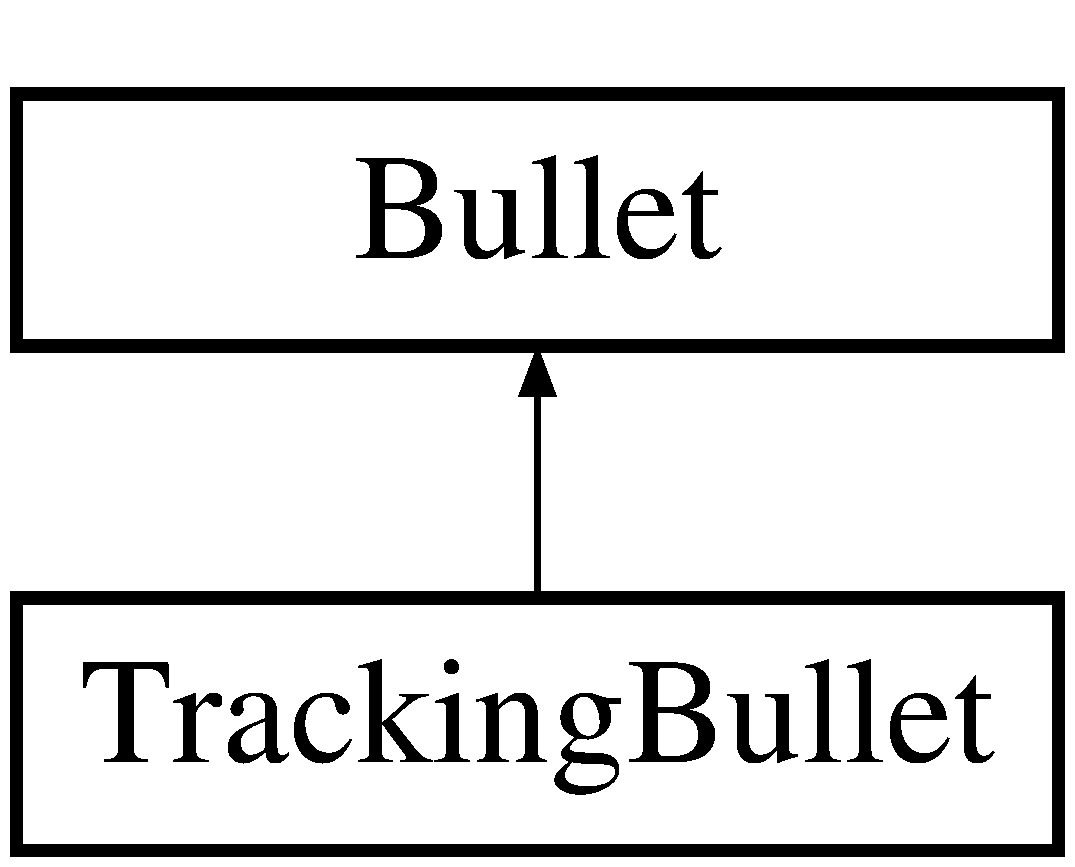
\includegraphics[height=2.000000cm]{class_tracking_bullet}
\end{center}
\end{figure}
\subsection*{Public Member Functions}
\begin{DoxyCompactItemize}
\item 
\mbox{\Hypertarget{class_tracking_bullet_abcfcaaa22d6f571037038f978d1ca79a}\label{class_tracking_bullet_abcfcaaa22d6f571037038f978d1ca79a}} 
{\bfseries Tracking\+Bullet} (sf\+::\+Vector2f, sf\+::\+Vector2f, bool)
\item 
\mbox{\Hypertarget{class_tracking_bullet_a0ef27cc3f807201c3b19ddc86460f09c}\label{class_tracking_bullet_a0ef27cc3f807201c3b19ddc86460f09c}} 
void {\bfseries update} (sf\+::\+Vector2f)
\item 
\mbox{\Hypertarget{class_tracking_bullet_a6567a9eba421686f91e2f1766de31954}\label{class_tracking_bullet_a6567a9eba421686f91e2f1766de31954}} 
sf\+::\+Vector2f {\bfseries Normalize} (sf\+::\+Vector2f)
\end{DoxyCompactItemize}
\subsection*{Additional Inherited Members}


The documentation for this class was generated from the following files\+:\begin{DoxyCompactItemize}
\item 
A\+I\+Defender\+Project/Tracking\+Bullet.\+h\item 
A\+I\+Defender\+Project/Tracking\+Bullet.\+cpp\end{DoxyCompactItemize}

%--- End generated contents ---

% Index
\backmatter
\newpage
\phantomsection
\clearemptydoublepage
\addcontentsline{toc}{chapter}{Index}
\printindex

\end{document}
